\newpage
\chapter{Code description}
Most of the entities are written in the code-writing technique called the two-process method, introduced by Jiri Gaisler.
The technique is described on the follwowing webpage:\\ "https://www.gaisler.com/doc/vhdl2proc.pdf".\\


The two-process method divides the code into two processes; one asynchronous process and one synchronous process. The algorithm to be run by the entity is located within the asynchronous block. The results of the asynchronous block gets registered in to the synchronous process. The asynchronous process uses variables to a wide extent. Record types are also widely used. A two-process entity can be seen in Figure \ref{fig:two_process}.



\begin{figure}                                                         \centering
   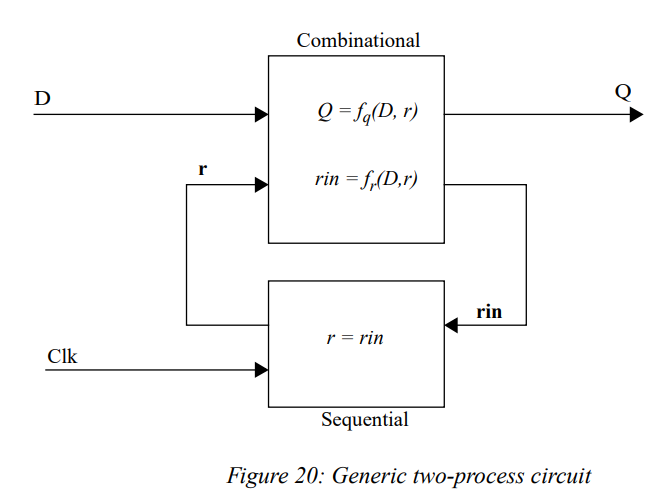
\includegraphics[scale=0.45]{images/two_process_method}
  \caption{ Two process method.} 
  \label{fig:two_process}
\end{figure}
 